\documentclass[10pt,letterpaper,twocolumn]{article}
% \usepackage[twocolumn]{geometry}
\usepackage{lmodern}% http://ctan.org/pkg/lm

% use Unicode characters
% try changing the option if you run into troubles with special characters
% (e.g. umlauts)
\usepackage[utf8x]{inputenc}
% clean citations
\usepackage{cite}
% hyperref makes references clicky.
\usepackage{nameref}
% line numbers
\usepackage[right]{lineno}
% improves typesetting in LaTeX
% \usepackage{microtype}
% degree symbol
\usepackage{gensymb}
\usepackage{amsmath}
\usepackage{booktabs}

% \DisableLigatures[f]{encoding = *, family = * }

% text layout - change as needed
% \raggedright{}
% \setlength{\parindent}{0.5cm}
% \textwidth 5.25in
% \textheight 8.75in

% Remove % for double line spacing
%\usepackage{setspace}
%\doublespacing

% use adjustwidth environment to exceed text width (see examples in text)
\usepackage{changepage}

% adjust caption style
\usepackage[aboveskip=1pt,labelfont=bf,
            labelsep=period,singlelinecheck=off]{caption}

% remove brackets from references
\makeatletter
\renewcommand{\@biblabel}[1]{\quad#1.}
\makeatother

% headrule, footrule and page numbers
\usepackage{lastpage,fancyhdr,graphicx}
\usepackage{epstopdf}
\pagestyle{myheadings}
\pagestyle{fancy}
\fancyhf{}
\rfoot{\thepage/\pageref{LastPage}}
\renewcommand{\footrule}{\hrule height 2pt \vspace{2mm}}
% \fancyheadoffset[L]{2.25in}
% \fancyfootoffset[L]{2.25in}

% use \textcolor{color}{text} for colored text (e.g. highlight to-do areas)
\usepackage{color}

% define custom colors (this one is for figure captions)
\definecolor{Gray}{gray}{.25}

% this is required to include graphics
\usepackage{graphicx}

% use if you want to put caption to the side of the figure - see example in text
\usepackage{sidecap}
% \usepackage[urlcolor  = blue]{hyperref}

% hyperurls packages:
\usepackage{xcolor}
\usepackage[colorlinks = true,
            linkcolor = blue,
            urlcolor  = blue,
            citecolor = blue,
            anchorcolor = blue]{hyperref}


% use for have text wrap around figures
\usepackage{wrapfig}
\usepackage[pscoord]{eso-pic}
\usepackage[fulladjust]{marginnote}
\reversemarginpar{}

% new commands
\newcommand{\cel}{\emph{C.~elegans}}
\newcommand{\fog}{\emph{\mbox{fog-2}}}
\newcommand{\ecol}{\emph{E.~coli}}

% gene numbers
\newcommand{\fogn}{1,881}
\newcommand{\agen}{5,592}
\newcommand{\interactionn}{1,318}
\newcommand{\coexpressed}{905}
\newcommand{\intersectn}{1,040}
\newcommand{\femalen}{405}

% tf numbers
\newcommand{\tfaging}{145}
\newcommand{\tffog}{60}
\newcommand{\tfinteraction}{36}

% number of genes in gold standard
\newcommand{\goldn}{1,056}
\newcommand{\goldfound}{506}
\newcommand{\goldpval}{$<10^{-38}$}

% website commands
\newcommand{\website}{
            \url{https://wormlabcaltech.github.io/Angeles_Leighton_2016/}
            }
\newcommand{\webref}{
\href{https://wormlabcaltech.github.io/Angeles_Leighton_2016/}{website}}

% more space between rows
\newcommand{\ra}[1]{\renewcommand{\arraystretch}{#1}}

\newcommand{\titleone}{The \cel{} female state: Decoupling the
transcriptomic effects of aging and sperm-status}

\title{
  \Large
  \textbf{\titleone}
}

\author{David Angeles-Albores\textsuperscript{1,$\dagger{}$}
\and{}
Daniel H.W. Leighton\textsuperscript{2,$\dagger{}$}
\and{}
Tiffany Tsou\textsuperscript{1}
\and{}
Tiffany H. Khaw\textsuperscript{1}
\and{}
Igor Antoshechkin\textsuperscript{3}
\and{}
Paul W. Sternberg\textsuperscript{1,*}
}

% document begins here
\begin{document}\sloppy{}
% \vspace*{0.35in}

% title goes here:
\twocolumn[

% title
\maketitle
% author info
\textbf{$\dagger$} These authors contributed equally to this work\\
\textbf{1} Department of Biology and Biological Engineering,
and Howard Hughes Medical Institute, Caltech, Pasadena, CA, 91125, USA\\
\textbf{2} Department of Human Genetics, Department of Biological Chemistry,
and Howard Hughes Medical Institute, University of California,
Los Angeles, Los Angeles, CA 90095, USA\\
\textbf{3} Department of Biology and Biological Engineering, Caltech,
Pasadena, CA, 91125, USA\\
\textbf{*} Corresponding author. Contact:pws@caltech.edu

\section*{Abstract}
\bf{}  Understanding genome and gene function in a whole organism requires us to
fully comprehend the life cycle and the physiology of the organism in question.
Although \cel{} is traditionally though of as a hermaphrodite, XX animals exhaust
their sperm and become (endogenous) females after 3 days of egg-laying. The
molecular physiology of this state has not been studied as intensely as other
parts of the life cycle, in spite of documented changes in behavior and
metabolism that occur at this stage. To study the female state of \cel{},
we designed an experiment to measure the transcriptomes of 1st day adult
females; endogenous, 6th day adult females; and at the same time points, mutant
feminized worms. At these time points, we were able to separate the effects of
biological aging from the transition into the female state.
We find that spermless young adult animals partially phenocopy 6 day old
wild-type animals that have depleted their sperm after egg-laying, and that
spermless animals also exhibit fewer differentially expressed genes as they age
throughout these 6 days. Our results indicate that sperm loss is responsible for
some of the naturally occuring transcriptomic changes that occur during the life
cycle of these animals.
These changes are enriched in transcription factors canonically associated with
neuronal development and differentiation. Our data provide a high-quality
picture of the changes that happen in global gene expression throughout the
period of early aging in the worm.\vspace{10mm}

]
% now start line numbers
\nolinenumbers{}

% the * after section prevents numbering
\section*{Introduction}
\label{sec:introduction}
% TODO cite wormbook “primer” chapter
Transcriptome analysis by RNA-seq~\cite{Mortazavi2008} has allowed for high
depth analysis of gene expression changes between life stages and environmental
conditions in many species~\cite{Gerstein2014,Blaxter2012}.
\emph{Caenorhabditis~elegans}, a genetic model nematode with extremely
well defined and largely invariant development~\cite{Sulston1977,Sulston1983},
has been subjected to extensive transcriptomic analysis across all stages of
larval development~\cite{Hillier2009,Boeck2016,Murray2012}
and many stages of embryonic development~\cite{Boeck2016}. Although RNA-seq was
used to develop transcriptional profiles of the mammalian aging process soon
after its invention~\cite{Magalhaes2010}, few such studies have been conducted
in \cel{} past the entrance into adulthood.

% TODO cite wormbook primer chapter
A distinct challenge to the study of aging transcriptomes in \cel{} is the
hermaphroditic lifestyle of wild-type individuals of this species. Young adult
hermaphrodites are capable of
self-fertilization~\cite{Brenner1974,corsi2015transparent}, and the resulting
embryos will contribute RNA to the resulting data.
Most previous attempts to study the \cel{} aging transcriptome have addressed
the aging process only indirectly, or relied on the use of genetically or
chemically sterilized animals to avoid this
problem~\cite{Murphy2003,Halaschek-wiener2005,Lund2002,McCormick2012,Eckley2013,
Boeck2016,Rangaraju2015}.
In addition, most of these studies obtained transcriptomes using microarrays,
which are less accurate than RNA-seq, especially for low-expressed
genes~\cite{Wang2014}.

Here, we investigate what we argue is a distinct state in the \cel{} life cycle,
the endogenous female state. Although \cel{} hermaphrodites emerge into adulthood
already replete with sperm, after about 3 days of egg-laying the animals become
sperm-depleted and can only reproduce by mating, This marks a transition into
what we define as the endogenous female state. This state is behaviorally
distinguished by increased male-mating success~\cite{Garcia2007}, which may be
due to an increased attractiveness to males~\cite{Morsci2011}. This increased
attractiveness acts at least partially through production of volatile chemical
cues~\cite{Leighton2014}.
% TODO (Wormbook “age related changes” chapter) cite
These behavioral changes are also coincident with functional deterioration of
the germline~\cite{Andux2008}, muscle~\cite{Herndon2002},
intestine~\cite{McGee2011} and nervous system~\cite{Liu2013}, changes
traditionally attributed to the aging process~\cite{golden2007gene}.

To decouple the effects of aging and sperm-loss, we devised a two factor
experiment. First, we examined wild type XX animals at the beginning of
adulthood (before worms contained embryos, referred to as 1st day adults) and
after sperm depletion (6 days after the last molt, which we term 6th day
adults). Second, we examined feminized XX animals that fail to produce sperm but
are fully fertile if supplied sperm by mating with males (see
Fig.~\ref{fig:wormlife}). We selected a mutant as a spermless worm suitable for
analysis. \fog{} is involved in germ-cell sex determination in the hermaphrodite
worm and is required for sperm production~\cite{Schedl1988,Clifford2000}.

\cel{} defective in sperm formation will never transition to a hermaphroditic
stage. As time moves forward, these spermless worms only exhibit changes
related to biological aging. We also reasoned that we might be able to identify
gene expression changes due to different life histories: whereas hermaphrodites
lay almost 300 eggs over three days, spermless females do not lay a single one.
The different life histories could affect gene expression.

Here, we show that we can detect a transcriptional signature associated both
with loss of hermaphroditic sperm and entrance into the endogenous female state.
We can also detect changes associated specifically with biological aging.
Loss of sperm leads to increases in the expression levels of transcription
factors that are canonically associated with development and cellular
differentiation and enriched in neuronal functions.
Biological aging also causes transcriptomic changes consisting of \agen{} genes
in \cel{}. 4,552 of these changes are common between wild-type and \fog{} worms,
indicating they do not depend on life history or genotype. To facilitate
exploration of the data, we have generated a website with interactive plots:
\website{}.

% figure experiment design
\begin{figure}[htbp]
\renewcommand{\familydefault}{\sfdefault}\normalfont{}
\centering
\captionsetup{width=\linewidth}
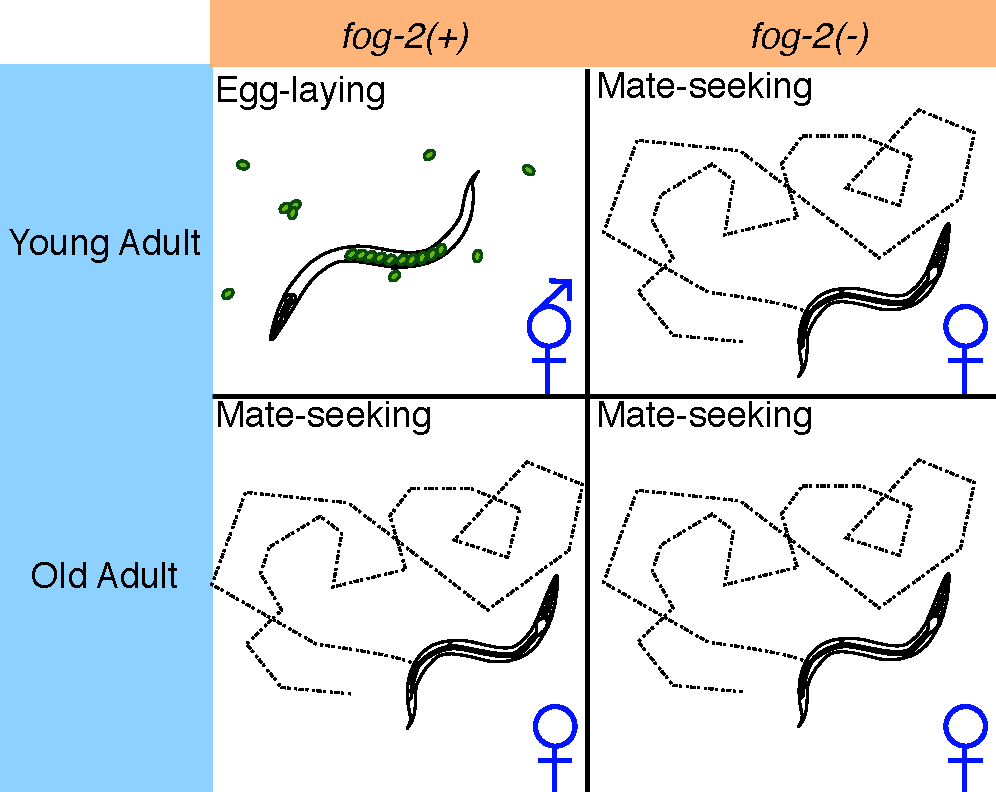
\includegraphics[width=\linewidth]{../output/figs/final_figs/worm_life_fog2_vs_n2.pdf}
\caption{Experimental design to identify genes associated with sperm loss and
with aging. Studying the wild-type worm alone would measure time- and
sperm-related changes at the same time, without allowing us to separate these
changes. Studying the wild-type worm and a \fog{} mutant would enable us to
measure sperm-related changes but not time-related changes. By mixing both
designs, we can measure and separate both modules.
}%
\label{fig:wormlife}
\end{figure}

\section*{Materials and Methods}
\label{sec:materials_methods}

\subsection*{Strains}
\label{sub:Strains}
Strains were grown at 20\degree{}C on NGM plates containing \ecol{} OP50. We
used the laboratory \cel{} strain N2 as our wild-type strain~\cite{Brenner1974}.
We also used the N2 mutant strain JK574, which contains the \fog{}\emph{(q71)}
allele, for our experiments.

\subsection*{RNA extraction}
\label{sb:rna_extraction}
Synchronized worms were grown to either young adulthood or the 6th day of
adulthood prior to RNA extraction. Synchronization and aging were carried out
according to protocols described previously~\cite{Leighton2014}. 1,000--5,000
worms from each replicate were rinsed into a microcentrifuge tube in S basal
(5.85g/L NaCl, 1g/L $\mathrm{K}_2\mathrm{HPO}_4$, 6g/L
$\mathrm{KH}_2\mathrm{PO}_4$), and then spun down at 14,000rpm for 30s. The
supernatant was removed and 1mL of TRIzol was added. Worms were lysed by
vortexing for 30~s at room temperature and then 20~min at 4\degree. The TRIzol
lysate was then spun down at 14,000rpm for 10~min at 4\degree{}C to allow
removal of insoluble materials. Thereafter the Ambion TRIzol protocol was
followed to finish the RNA extraction (MAN0001271 Rev. Date: 13 Dec 2012).
3 biological replicates were obtained for each genotype and each time point.

\subsection*{RNA-Seq}
\label{sb:rna_seq}
RNA integrity was assessed using RNA 6000 Pico Kit for Bioanalyzer (Agilent
Technologies \#5067--1513) and mRNA was isolated using NEBNext Poly(A) mRNA
Magnetic Isolation Module (New England Biolabs, NEB, \#E7490). RNA-Seq libraries
were constructed using NEBNext Ultra RNA Library Prep Kit for Illumina (NEB
\#E7530) following manufacturer’s instructions. Briefly, mRNA isolated from
$\sim1\mu$g of total RNA was fragmented to the average size of 200 nt by
incubating at 94 °C for 15 min in first strand buffer, cDNA was synthesized
using random primers and ProtoScript II Reverse Transcriptase followed by
second strand synthesis using Second Strand Synthesis Enzyme Mix (NEB).
Resulting DNA fragments were end-repaired, dA tailed and ligated to NEBNext
hairpin adaptors (NEB \#E7335).
After ligation, adaptors were converted to the ‘Y’ shape by treating with USER
enzyme and DNA fragments were size selected using Agencourt AMPure XP beads
(Beckman Coulter \#A63880) to generate fragment sizes between 250 and 350 bp.
Adaptor-ligated DNA was PCR amplified followed by AMPure XP bead clean up.
Libraries were quantified with Qubit dsDNA HS Kit (ThermoFisher Scientific
\#Q32854) and the size distribution was confirmed with High Sensitivity DNA Kit
for Bioanalyzer (Agilent Technologies \#5067--4626).
Libraries were sequenced on Illumina HiSeq2500 in single read mode with the read
length of 50 nt following manufacturer's instructions. Base calls were performed
with RTA 1.13.48.0 followed by conversion to FASTQ with bcl2fastq 1.8.4.


% \subsection*{RNA interference}
% \label{sb:rnai}
% RNAi was performed as described in previous protocols~\cite{Kamath2001} using a commercially available RNAi library~\cite{Kamath2003}. RNAi bacterial strains were grown in LB plus 100$\mu$g/mL ampicillin overnight. Fresh RNAi cultures were then plated onto NGM agar plates containing 25$\mu$g/mL carbenicillin and 1mM IPTG\@. N2 or \fog{}\emph{(q71)} hermaphrodites grown on \ecol{} OP50 were bleached onto NGM plates without \ecol{}, and allowed to hatch and develop into L1 larvae. Starved L1s were transferred to recently seeded RNAi plates.
% All assays were performed on the offspring of these L1s (F1 generation). Worms grown on every RNAi strain were monitored for gross abnormalities, such as sterility, lethality and larval arrest. Control worms in all assays were fed with an \mbox{anti-\emph{gfp}} RNAi strain. All RNAi-treated worms were grown at 20\degree{} C. We extracted plasmid DNA from all RNAi strains that showed a statistically significant phenotype to verify the sequence identity of the hits.

% \subsection*{Ovulation assay}
% \label{sb:oocyte_assay}
% We performed a slightly modified ovulation assay based on previously described protocols~\cite{White2012}. Feminized \fog{}\emph{(q71)} hermaphrodites were picked as virgin L4s the day before the assay to a fresh RNAi plate. The following day, the adult animals were placed on assay plates (6cm diameter plates, NGM agar seeded with 15$\mu$L of \ecol{} OP50 four days earlier), twenty worms per assay, and allowed to incubate at room temperature. Laid oocytes were counted after two hours. Plates were then left at room temperature overnight to serve as lawn-leaving assays.
%
% \subsection*{Lawn-leaving assay}
% \label{sb:lawn_leaving}
% Lawn-leaving assays were performed as described previously~\cite{Lipton2004}. Young adult N2 hermaphrodites were selected the day of the assay and placed on assay plates (same as the ovulation assay plates), twenty worms per assay, and allowed to incubate at room temperature overnight. Assays for \fog{}\emph{(q71)} were performed on the same worms as used in the ovulation assay. The following morning, plates were scored for leaving, with any worm touching any part of the bacterial lawn with any part of its body deemed to be “on” the lawn, and all others deemed to be “off”.

% \subsection*{Brood size counting}
% \label{sb:brood_size}
% Worms were selected for this assay as L4 hermaphrodites to ensure that all progeny could be counted. For each replicate of each assay, a single worm was placed on a fresh RNAi plate and incubated at 20\degree{}C. Every 1--2 days, the test worm was moved to a fresh RNAi plate, until it stopped laying eggs. Progeny were counted on each plate before they reached adulthood to ensure that only a single generation was counted.

\subsection*{Statistical Analysis}
\label{sb:statistics}
\subsubsection*{RNA-Seq Analysis.}
\label{sb:model}
RNA-Seq alignment was performed using Kallisto~\cite{Bray2016} with 200
bootstraps. The commands used for read-alignment are in the S.I. file 1.
Differential expression analysis was performed using Sleuth~\cite{Pimentel2016}.
The following General Linear Model (GLM) was fit:

\begin{align*}
  \log(y_i) =& \beta_{0,i} + \beta_{G,i}\dot~G + \\
  &\beta_{A,i}\dot~A + \beta_{A::G,i}\dot~A~G,
  \label{eqn:GLM}
\end{align*}

where $y_i$ are the TPM counts for the ith gene; $\beta_{0,i}$ is the intercept
for the ith gene, and $\beta_{X,i}$ is the regression coefficient for variable
$X$ for the $i$th gene; $A$ is a binary age variable indicating 1st day adult
(0) or 6th day adult (1) and $G$ is the genotype variable indicating wild-type
(0) or \fog{} (1); $\beta_{A::G, i}$ refers to the regression coefficient
accounting for the interaction between the age and genotype variables in the
$i$th gene. Genes were called significant if the FDR-adjusted q-value for any
regression coefficient was less than 0.1. Our script for differential analysis
is available on GitHub.

Regression coefficients and TPM counts were processed using Python 3.5 in a
Jupyter Notebook~\cite{Perez2007}. Data analysis was performed using the Pandas,
NumPy and SciPy libraries~\cite{McKinney2011,VanDerWalt2011,Oliphant2007}.
Graphics were created using the Matplotlib and Seaborn
libraries~\cite{Waskom,Hunter2007}. Interactive graphics were generated using
Bokeh~\cite{Team2014}.

Tissue, Phenotype and Gene Ontology Enrichment
Analyses (TEA, PEA and GEA, respectively) were performed using the WormBase
Enrichment Suite for Python~\cite{Angeles-Albores2016}.

% \subsubsection*{Brood Size Analysis.}
% Brood size results were analyzed using Welch's t-test to identify RNAi treatments that were significantly different from a \emph{gfp} RNAi control. RNAi control results were pooled over multiple days because we could not detect systematic day-day variation. We did not apply FDR or Bonferroni correction because, at a p-value threshold for significance of 0.05, we expected 1 false positive on average per screen.

% \subsubsection*{Lawn-leaving Analysis.}
% Lawn-leaving results were analyzed using a $\chi^2$ test for categorical variables. Results were considered statistically significant if $p<0.05$. No FDR or Bonferroni correction was applied because the size of the screen was too small, with 1 false positive expected on average per screen. However, the lawn-leaving results suffered from high variance, which can lead to false positive results.
% To safeguard against false positive discovery, we used a non-parametric bootstrap to estimate the true $\chi^2$ value. Using a bootstrap on this dataset does not lead to statistical acceptance of any gene that was not accepted without a bootstrap; however, applying a boostrap does lead to statistical rejection of a large number of results.
%
% \subsubsection*{Ovulation Assay Analysis.}
% Ovulation assay results were analyzed using a non-parametric bootstrapped Mann-Whitney U-test because the \emph{gfp} control variance was very large relative to the variance of the RNAi treatments. Results were considered statistically significant if $p<0.05$.


\subsection*{Data Availability}
\label{sb:data_availability}
Strains are available from the \emph{Caenorhabditis} Genetics Center upon
request. All of the data and scripts pertinent for this project except the raw
reads can be found on our Github repository
\url{https://github.com/WormLabCaltech/Angeles_Leighton_2016}. File S1 contains
the Kallisto commands used to process the read alignments as well as the
accession numbers for the raw-reads, whcih are available at GenBank. It also
contains a detailed explanation for the format of files S2 and S3. File S2
contains the list of genes that were altered in aging regardless of genotype.
File S3 contains the list of genes and their associations with the \fog{}
phenotype. File S4 contains the genes that changed differently in aging
wild-type worms and in \fog{} mutants. Raw reads will be deposited in the
Sequence Read Archive and made available shortly.

\section*{Results}
\label{sec:results}
% figure (aging transcriptomics)
\begin{figure}[htbp]
\renewcommand{\familydefault}{\sfdefault}\normalfont{}
\centering
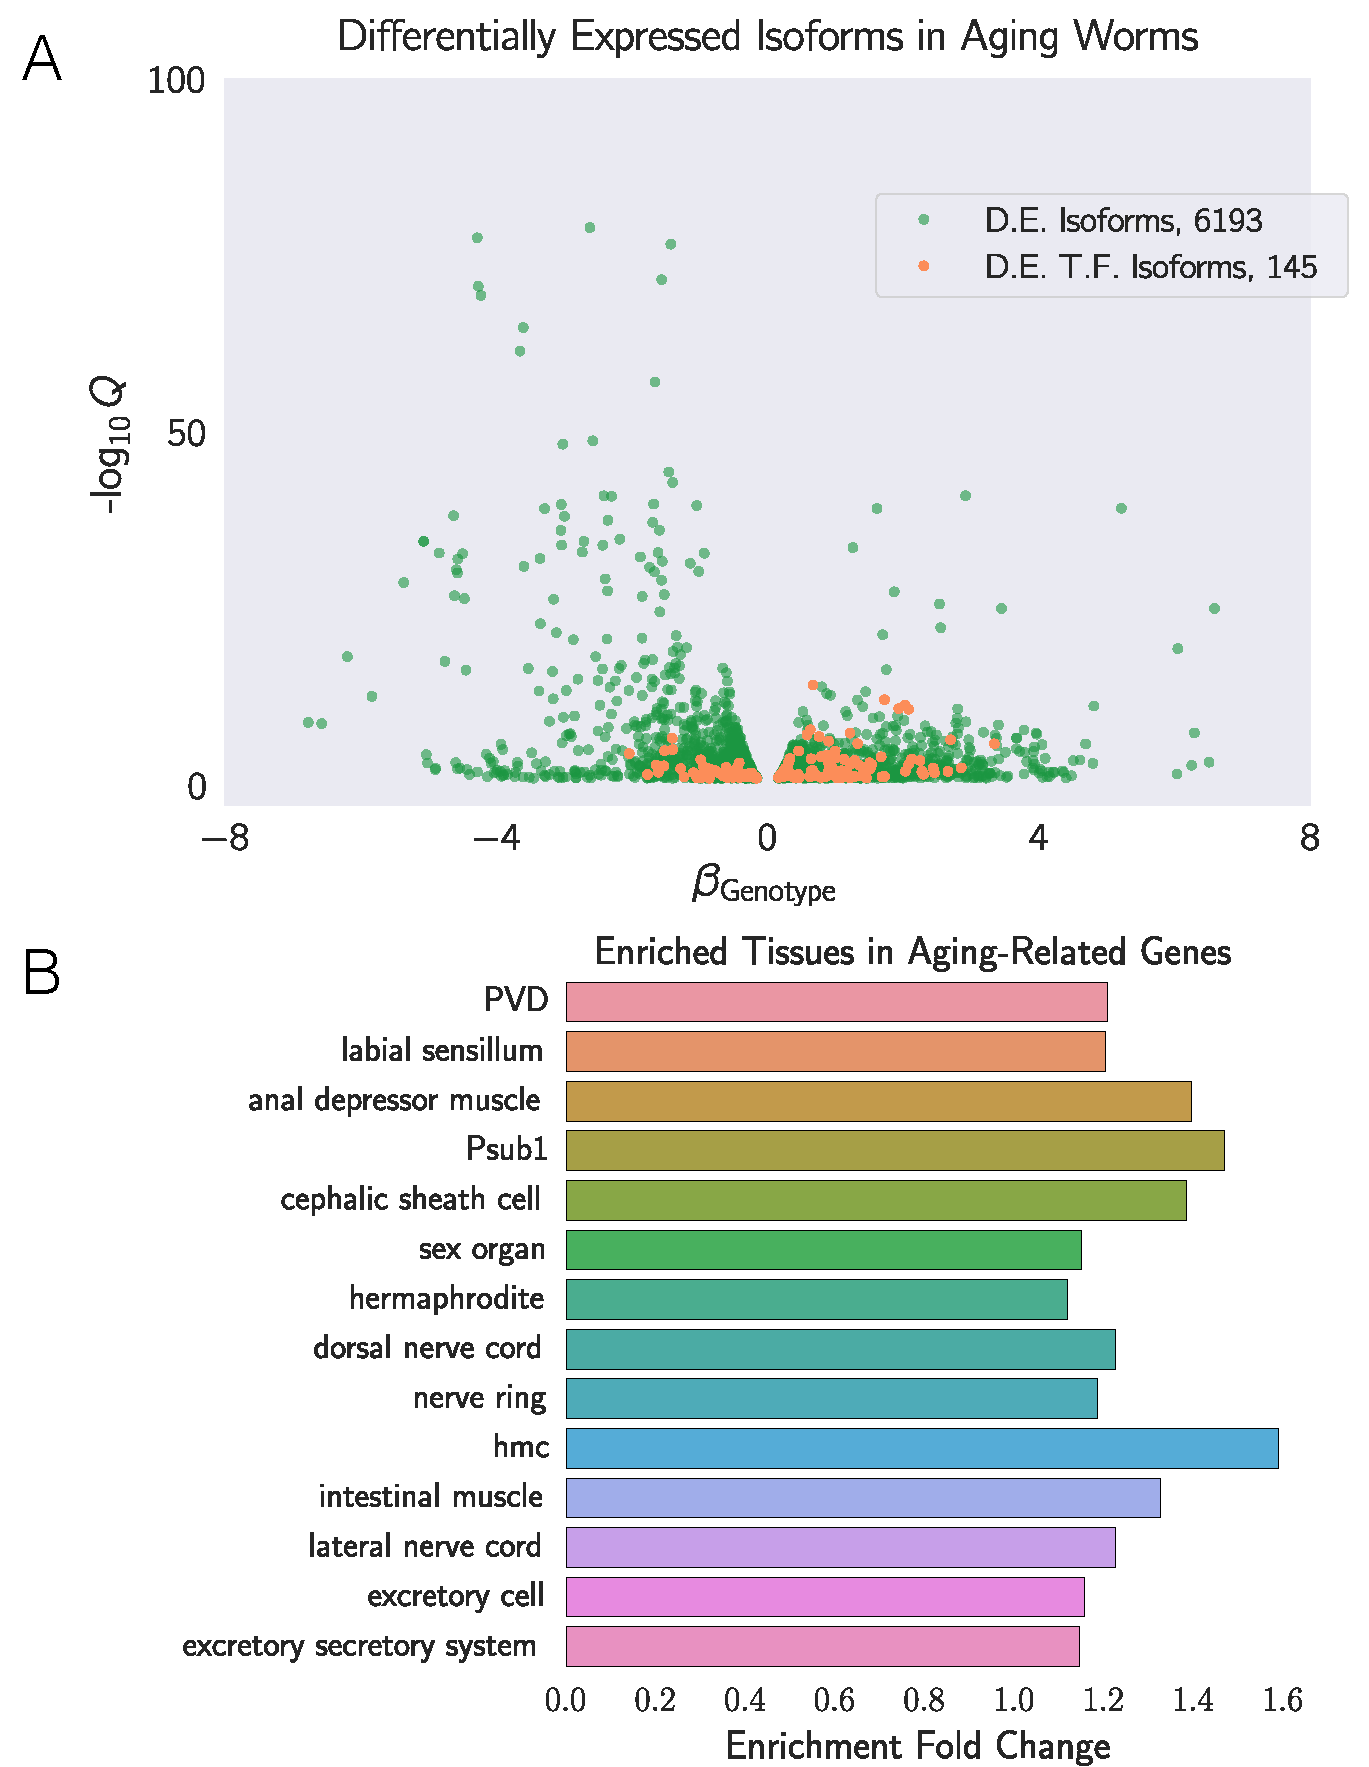
\includegraphics[width=\linewidth]{../output/figs/final_figs/aging_transcriptomics.pdf}
\caption{\textbf{A} We identified a common aging transcriptome between N2 and
\fog{} animals, consisting of 6,193 differentially expressed isoforms totaling
\agen{} genes. The volcano plot is randomly down-sampled 30\% for ease of
viewing. Each point represents an individual isoform. $\beta{}_\mathrm{Aging}$
is the regression coefficient. Larger magnitudes of $\beta$ indicate a larger
log-fold change. The y-axis shows the negative logarithm of the q-values for
each point. Green points are differentially expressed isoforms; orange points
are differentially expressed isoforms of  predicted transcription factor
genes~\cite{Reece-Hoyes2005}. An interactive version of this graph can be found
on our \webref{}. \textbf{B} Tissue Enrichment
Analysis~\cite{Angeles-Albores2016} showed that genes associated with muscle
tissues and the nervous system are enriched in aging-related genes.
Only statistically significantly enriched tissues are shown. Enrichment Fold
Change is defined as $Observed/Expected$.\ hmc stands for head mesodermal cell.
}
\label{fig:agingtranscriptome}
\end{figure}

\subsection*{Decoupling time-dependent effects from sperm-status via general
linear models}
\label{sub:Transcriptomics}
In order to decouple time-dependent effects from changes associated with loss
of hermaphroditic sperm, we measured wild-type and \fog{} adults at the 1st day
adult stage (before visible embryos were present) and 6th day adult stage, when
all wild-type hermaphrodites had laid all their eggs (see
Fig~\ref{fig:wormlife}), but mortality is still low
($<10\%$)~\cite{Stroustrup2013}.  We obtained 16--19 million reads mappable to
the \cel{} genome per biological replicate, which enabled us to identify
14,702 individual genes totalling 21,143 isoforms (see
Figure~\ref{fig:agingtranscriptome}a).

\begin{figure}[htbp]
\renewcommand{\familydefault}{\sfdefault}\normalfont{}
\centering
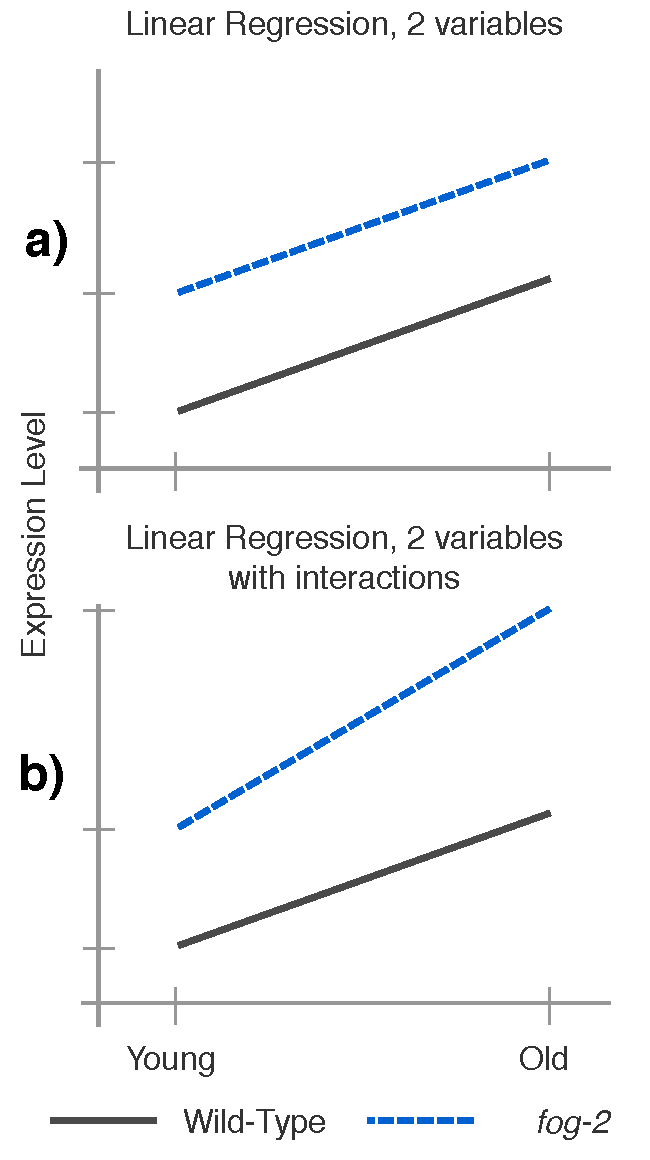
\includegraphics[width=0.9\linewidth]{../output/figs/final_figs/linear_regression.pdf}
\caption{\textbf{A} A linear regression with two variables, age and genotype.
The expression level of a gene increases by the same amount as worms age
regardless of genotype. However, \fog{} has more mRNA than the wild-type at all
stages (blue arrow). \textbf{B} A linear regression with two variables and an
interaction term. In this example, the expression level of this hypothetical
gene is different between wild-type worms and \fog{} (blue arrow). Although the
expression level of this gene increases with age, the slope is different between
wild-type and \fog{}. The difference in the slope can be accounted for through
an interaction coefficient (red arrow).
}
\label{fig:linear_reg}
\end{figure}

One way to analyze the data from this two-factor design is by pairwise
comparison of the distinct states. However, such an analysis would not make full
use of all the statistical power afforded by this experiment. Another method
that makes full use of the information in our experiment is to perform a linear
regression in 3 dimensions (2 independent variables, age and genotype, and 1
output). A linear regression with 1 parameter (age, for example) would fit a
line between expression data for young and old animals. When a second parameter
is added to the linear regression, said parameter can be visualized as altering
the y-intercept, but not the slope, of the first line in question (see
Fig.~\ref{fig:linear_reg}a).

Although a simple linear model is oftentimes useful, sometimes it is not
appropriate to assume that the two variables under study are entirely
independent. For example, in our case, three out of the four timepoint and
genotype combinations we studied did not have sperm, and sperm-status is
associated with both the \fog{} self-sterile phenotype and with biological age
of the wild-type animal. One way to statistically model such correlation between
variables is to add an interaction term to the linear regression.
This interaction term allows extra flexibility in describing how changes occur
between conditions. For example, if age increased the expression of a
theoretical gene \emph{X} in a wild-type animal, and if that same gene was
altered in a \fog{} animal, but the increase in the levels of gene \emph{X} in
\fog{} is much, much greater than in the wild-type, then we could add a positive
interaction coefficient to the model to explain the effect of genotype on the
y-intercept as well as the slope (see Fig.~\ref{fig:linear_reg}b). Likewise, if
the levels of \emph{X} in a \fog{} animal did not change with age, but if we
were certain that gene \emph{X} increases its expression with age in the
wild-type, then we could add a negative interaction term to the model to signal
that the genotype affected the slope of the animal.

For these reasons, we used a linear generalized model (see \nameref{sb:model})
with interactions to identify a transcriptomic profile associated with the
\fog{} genotype independently of age, as well as a transcriptomic profile of
\cel{} aging common to both genotypes. The change associated with each variable
is referred as $\beta$; this number, although related to the natural logarithm
of the fold change, is not exactly equal to it. However, it is true that larger
magnitudes of $\beta$ indicate greater change. Thus, for each gene we performed
a linear regression, and we evaluated the whether the $\beta$ values associated
with each coefficient were significantly different from 0 via a Wald test
corrected for multiple hypothesis testing. A coefficient was considered to be
significantly different from 0 if the q-value associated with it was less than
0.1.

\subsubsection*{A quarter of all genes change expression between the 1st day of
                adulthood and the 6th day of adulthood in \cel{}.}
% We identified a transcriptomic signature consisting of \agen{} genes that were
% differentially expressed in 6th day adult animals of either genotype relative
% to 1st day adult animals (see SI file 2). This constitutes more than one quarter
% of the genes in \cel{}. Tissue Enrichment Analysis
% (TEA)~\cite{Angeles-Albores2016} showed that muscle- and hypodermis-associated
% genes are particularly enriched in this dataset (see
% Figure~\ref{fig:agingtranscriptome}b). Gene ontology analysis using
% PEA revealed that genes that were differentially expressed during the course of
% aging were enriched in terms related to metabolism
% (TCA;\@ cellular amino acid catabolic process; purine nucleobase metabolic
% process; respiratory electron transport chain) as well as gene signaling
% (oxidative phosphorylation; regulation of gene expression, epigenetic).
We identified a transcriptomic signature consisting of \agen{} genes that were
differentially expressed in 6th day adult animals of either genotype relative
to 1st day adult animals (see SI file 2). This constitutes more than one quarter
of the genes in \cel{}. Tissue Enrichment Analysis
(TEA)~\cite{Angeles-Albores2016} showed that
nervous tissues including the `nerve ring', `dorsal nerve cord', `PVD' and
`labial sensillum' were enriched in genes that become differentially expressed
through aging. Likewise, certain muscle groups (`anal depressor muscle',
`intestinal muscle') were enriched.
(see Figure~\ref{fig:agingtranscriptome}b). Gene Enrichment Analysis
(GEA)~\cite{} revealed that genes that
were differentially expressed during the course of
aging were enriched in terms involving respiration (`respiratory
chain', `oxoacid metabolic process'); translation (`cytosolic large
ribosomal subunit'); and nucleotide metabolism (`purine nucleotide', `nucleoside
phosphate' and `ribose phosphate' metabolic process). Phenotype Enrichment
Analysis (PEA)~\cite{} showed enrichment
of phenotypes that affect the \cel{} gonad, including `gonad vesiculated',
`gonad small', `oocytes lack nucleus' and `rachis narrow'.

To verify the quality of our dataset, we generated a list of \goldn{} golden
standard genes expected to be altered in 6th day adult worms using previous
literature reports including downstream genes of \emph{daf-12}, \emph{daf-16},
and aging and lifespan extension datasets~\cite{Murphy2003,Halaschek-wiener2005,
Lund2002,McCormick2012,Eckley2013}. Out of \goldn{} standard genes, we found
\goldfound{} genes in our time-responsive dataset. This result was statistically
significant with a p-value \goldpval{}.

% \begin{table*}
% \renewcommand{\familydefault}{\sfdefault}\normalfont{}
% \centering{}
% \ra{1.3}
% \caption{\textbf{Transcription Factor TEA Results.} We ran TEA on the
% transcription factors associated with aging. Raw results showed a large list of
% terms associated with embryonic tissues that are neuronal precursors (AB
% lineage), so we trimmed the results by removing any terms that were expected to
% show up less than once in our list (if a term is expected to show up $10^{-3}$
% times in a list, 1 occurrence is enough to show enrichment in this list,
% leading to many false positives). The best 5 results by Q-value are shown below.}
% \begin{tabular}{@{}lccr@{}}
% \toprule{}
% Tissue & Expected & Observed & Q-value\\
% \bottomrule{}\\
% % P11 & 1 & 9 & $<10^{-5}$\\
% % ventral nerve cord &	9 &	26 &	$<10^{-5}$\\
% % dorsal nerve cord &	5 &	19 & $<10^{-5}$\\
% % head muscle & 3	& 13 &	$<10^{-4}$\\
% % P7.p & 1 &	6	& $<10^{-2}$\\
% \bottomrule{}
% \end{tabular}
% \label{tab:tea_tf_age}
% \end{table*}

Next, we used a published compendium~\cite{Reece-Hoyes2005} to search for known
or predicted transcription factors. We found \tfaging{} transcription factors in
the set of genes with differential expression in aging nematodes. We subjected
this list of transcription factors to TEA to understand their expression
patterns. 6 of these
transcription factors were expressed in the `hermaphrodite specific neuron'
(HSN), a neuron physiologically relevant for egg-laying (\emph{hlh-14}, \emph{sem-4},
\emph{ceh-20}, \emph{egl-46}, \emph{ceh-13}, \emph{hlh-3}), which represented
a statistically significant 2-fold enrichment of this tissue ($q<10^{-1}$).
The term `head muscle' was also overrepresented at twice the expected level
($q<10^-1$, 13 genes). Many of these transcription factors
have been  associated with developmental processess, and it is unclear why they
would change expression in adult animals. Interactive volcano plots for each
gene-set can be found in our \webref{}.

\subsubsection*{The whole-organism \fog{} transcriptome in \cel{}.}

We were also able to identify \fogn{} genes associated with the \fog{} genotype,
including \tffog{} transcription factors (see SI file 3).
% Gonad-related tissues
% were enriched in this gene set (midbody; somatic gonad, $q<0.1$
% for all), consistent with the function of \fog{} as a sperm specification factor
TEA showed that the terms `AB', `midbody', `uterine muscle', `cephalic sheath
cell', `anal depressor muscle' and `PVD' were enriched in this gene set. The
terms `AB' and `midbody' likely reflect the impact of \fog{} on the germline
(see Jupyter Notebook, section on
\href{https://wormlabcaltech.github.io/Angeles_Leighton_2016/RNASeqAnalysis.html#Run-TEA}{Tissue Enrichment Analysis}).
% Gene Ontology analysis using the PANTHER GO-Slim Celluar Component
% dataset~\cite{Mi2009} showed that this dataset was enriched in terms related to
% metabolism (TCA;\@ generation of precursor metabolites and energy; lipid
% metabolic process), and in cell division (mitosis). Additionally, this dataset
% was depleted for genes annotated with the term `sensory perception of chemical
% stimulus'.
% Similarly to the transcription factors associated with aging, tissue
% enrichment analysis of these transcription factors reveals that they are involved
% in neural development.
Phenotype enrichment showed that only a single phenotype, `spindle orientation
variant' was enriched in the \fog{} transcriptome ($q<10^{-1}$, 38 genes, 2-fold
enrichment). Most genes annotated as `spindle orientation variant' were
slightly upregulated, and therefore are unlikely to uniquely reflect reduced
germline proliferation. GO term enrichment was very similar to the aging gene
set and reflected enrichment in annotations pertaining to translation and
respiration. Unlike the aging gene set, the \fog{} transcriptome was
significantly enriched in `myofibril' and `G-protein coupled receptor binding'
($q<10^{-1}$). Enrichment of the term `G-protein coupled receptor binding' was
due to 14 genes: \emph{cam-1}, \emph{mom-2},  \emph{dsh-1}, \emph{spp-10},
\emph{flp-6}, \emph{flp-7}, \emph{flp-9}, \emph{flp-13}, \emph{flp-14},
\emph{flp-18},
\emph{K02A11.4}, \emph{nlp-12}, \emph{nlp-13}, and \emph{nlp-40}.
\emph{dsh-1},
\emph{mom-2} and \emph{cam-1} are members of the Wnt signaling pathway.
Most of these genes were up-regulated, suggesting increased G-protein binding
activity in \fog{} mutants.

Of the \fogn{} genes that we identified in the \fog{}
transcriptome, \intersectn{} genes were also identified in our aging set.
Moreover, of these \intersectn{}  genes, \coexpressed{} genes changed in the
same direction in response either aging or germline feminization.
We were surprised at the large fraction of genes that overlapped between these
two categories. Such a large overlap is indicative of correlations between aging
and sperm-loss. There are four possibilities. First, the \fog{} mutant worms may
have a fast-aging phenotype, in which case the interaction coefficients should
match the sign of the aging coefficient. Second, the \fog{} mutant worms may
have a slow-aging phenotype, in which case the interaction coefficients should
have an interaction coefficient that is of opposite sign, but not greater
magnitude than the aging coefficient (if a gene increases in aging in a
wild-type worm, it should still increase in a \fog{} worm, albeit more slowly).
Third, the \fog{} worms exhibit a rejuvenation phenotype. If this is the case,
then these genes should have an interaction coefficient that is of opposite sign
and greater magnitude than their aging coefficient, such that the change of
these genes in \fog{} mutant worms is reversed relative to the wild-type.
Finally, if these genes are indicative of a female state, then these genes
should not change with age in \fog{} animals, since these animals do not exit
this state during the course of the experiment. Moreover, because wild-type
worms become female as they age, a further requirement for a transcriptomic
signature of the female state is that aging coefficients for genes in this
signature should have genotype coefficients of equal sign and magnitude. In
other words, entrance into the female state should be not be path-dependent.

% aberrant aging
\begin{figure}
\renewcommand{\familydefault}{\sfdefault}\normalfont{}
\centering
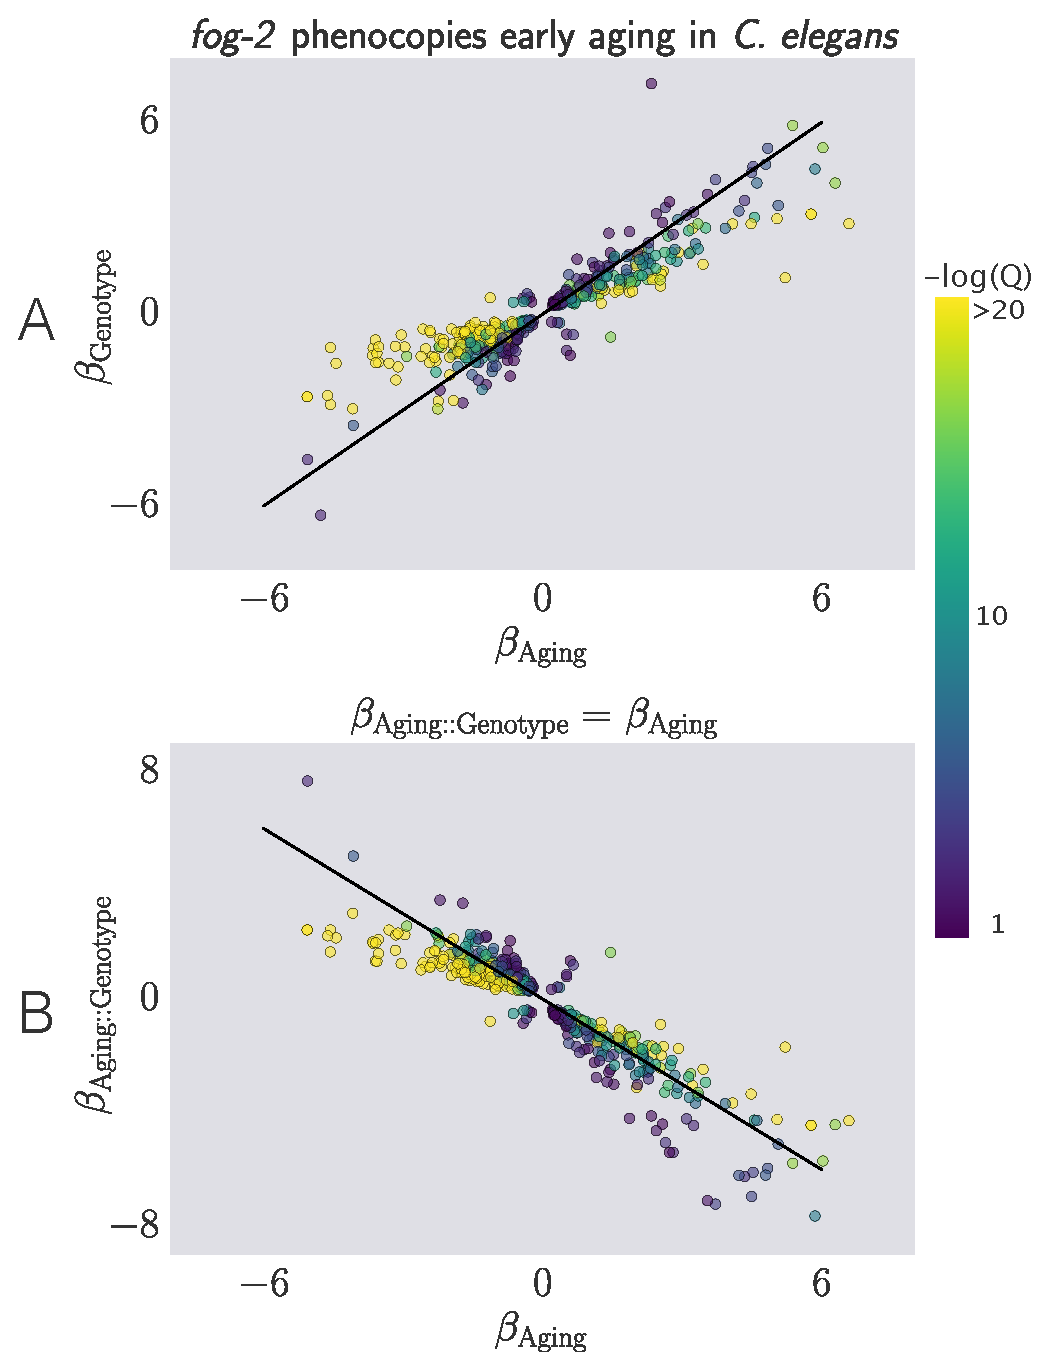
\includegraphics[width=\linewidth]{../output/figs/final_figs/aberrant_aging.pdf}
\caption{
\fog{} partially phenocopies early aging in \cel{}. The $\beta$ in
each axes is the regression coefficient from the GLM, and can be loosely
interpreted as an estimator of the log-fold change.
Feminization by loss of \fog{} is associated with a transcriptomic phenotype
involving \fogn{} genes. \intersectn{}/\fogn{} of these genes are also altered
in wild-type worms as they progress from young adulthood to old adulthood, and
\coexpressed{} change in the same direction. However, progression from young to
old adulthood in a \fog{} background results in no change in the expression
level of these genes. \textbf{A} We identified genes that change similarly in
feminization as in aging. Black line is the line $y=x$, not a line of best fit.
\textbf{B} Many of the genes in \textbf{A} do not further change with age in a
\fog{} animal.
The black line is the line $y=-x$, and is not a line of best fit. Color is
proportional to $-\log{Q}$.
An interactive version of these graphs can be found on our \webref{}.
}%
\label{fig:aberrant_aging}
\end{figure}

To evaluate which of these possibilities was most likely to be true, we selected
the \intersectn{} genes that had aging coefficients, genotype coefficients and
interaction coefficients significantly different from zero and we plotted their
temporal coefficients against their genotype coefficients (see
Fig.~\ref{fig:aberrant_aging}a). We observed a striking correlation between
aging and genotype coefficients. Most of these genes fell near the line $y=x$,
suggesting that these genes define a female state. As a further test that these
genes actually define a female state, we plotted the temporal coefficient
against the interaction coefficient for each gene.
This time, we observed an inverse correlation between the aging coefficients
and the interaction coefficients for this gene set. Overall, we identified
\femalen{} genes that increased in the same direction through age or mutation
of the \fog{} gene and that had an interaction coefficient of opposite sign to
the aging or genotype coefficient (see SI file 4). Taken together, this
information suggests that these \femalen{} genes define a female state in
\cel{}.

\subsection*{Analysis of the Female State Transcriptome}
% \begin{table*}
% \renewcommand{\familydefault}{\sfdefault}\normalfont{}
% \centering{}
% \ra{1.3}
% \caption{
% \textbf{Gene Ontology Enrichment.} Gene Ontology Enrichment Analysis
% was performed using PantherDB~\cite{Mi2009} on genes associated with the female
% state. The terms reflect changes in translational machinery. On the other hand,
% this list was depleted in genes that tend to be associated with sensory
% perception.
% }
% \begin{tabular}{@{}lccr@{}}
% \toprule{}
% Term & Expected & Observed & P-value\\
% \bottomrule{}\\
% Translation & 5 & 17 & $8.63\times{}10^{-3}$\\
% Proteolysis &	10 &	24 &	$1.12\times{}10^{-2}$\\
% Sensory Perception &	15 &	2 & $4.97\times{}10^{-3}$\\
% \bottomrule{}
% \end{tabular}
% \label{tab:female_go}
% \end{table*}

\begin{figure}
  \renewcommand{\familydefault}{\sfdefault}\normalfont{}
  \centering
  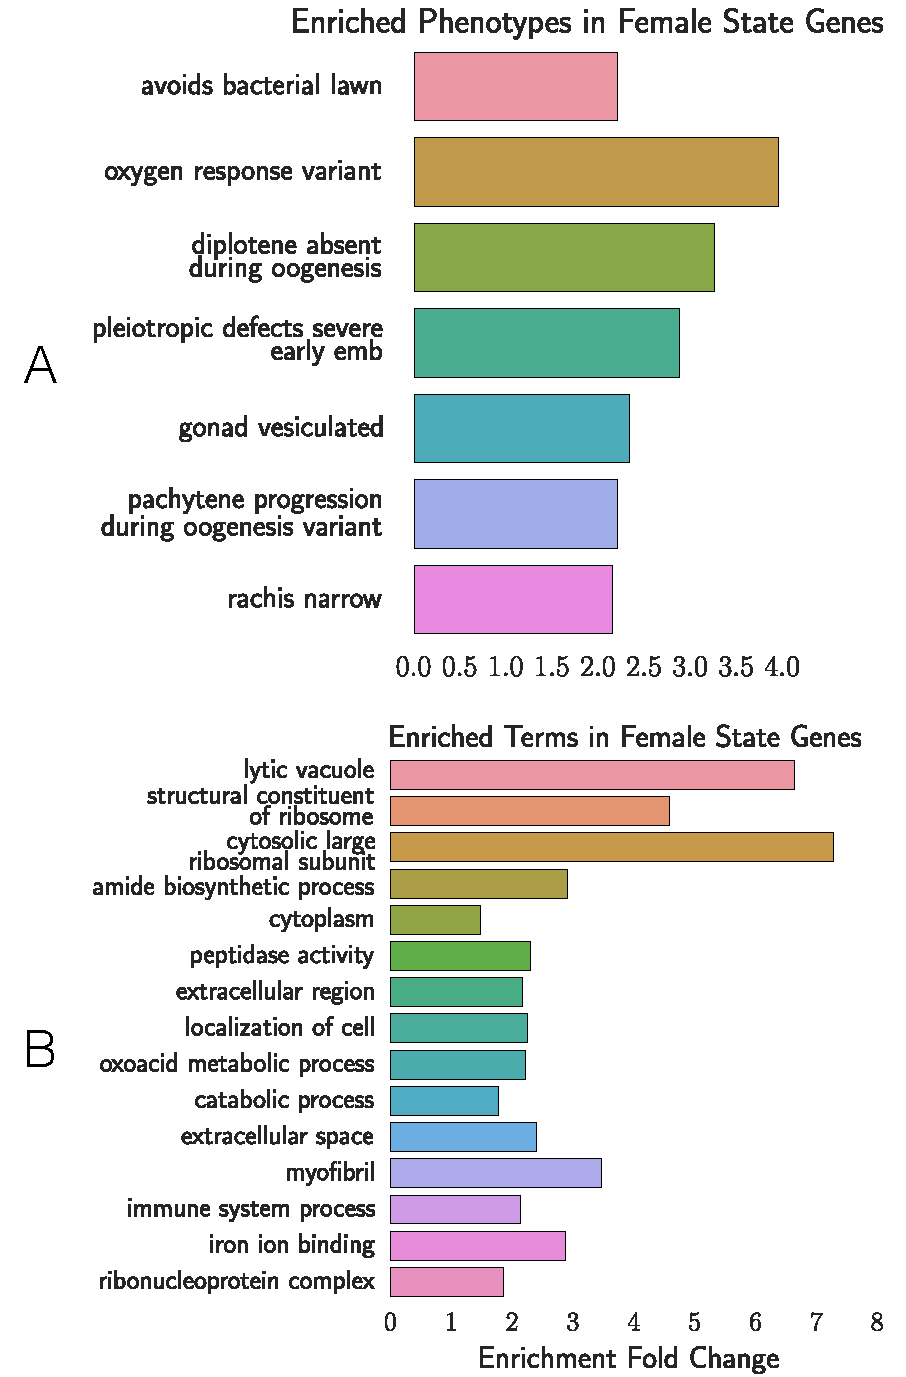
\includegraphics[width=0.9\linewidth]{../output/figs/final_figs/female_state_enrichment.pdf}
  \caption{
  Phenotype and GO enrichment of genes involved in the female state.
  \textbf{A}. PEA.
  \textbf{B}. GEA.
  Most of the terms enriched in PEA reflect the abundance of ribosomal subunits
  present in this gene set.
  }
\label{fig:female_state_enrich}
\end{figure}

To better understand the changes that happen after sperm loss, we performed
tissue enrichment, phenotype enrichment and gene ontology enrichment analyses
on the set of \femalen{} genes that we associated with the female state.
TEA showed no tissue enrichment using this gene-set. GEA
showed that this gene list was enriched in constituents of the ribosomal
subunits almost four times above background ($q<10^{-5}$, 17 genes). The
enrichment of ribosomal constituents in this gene set in turn drives the
enriched phenotypes: `avoids bacterial lawn',
`diplotene absent during oogenesis', `gonad vesiculated', `pachytene progression
during oogenesis variant', and `rachis narrow'. The expression of most of these
ribosomal subunits is down-regulated in aged animals or in \fog{} mutants.

% \subsection*{Screens}
% \label{subs:Screens}
%
% % figure 3 (brood assay)
% \begin{figure}
% \renewcommand{\familydefault}{\sfdefault}\normalfont{}
% \centering
% 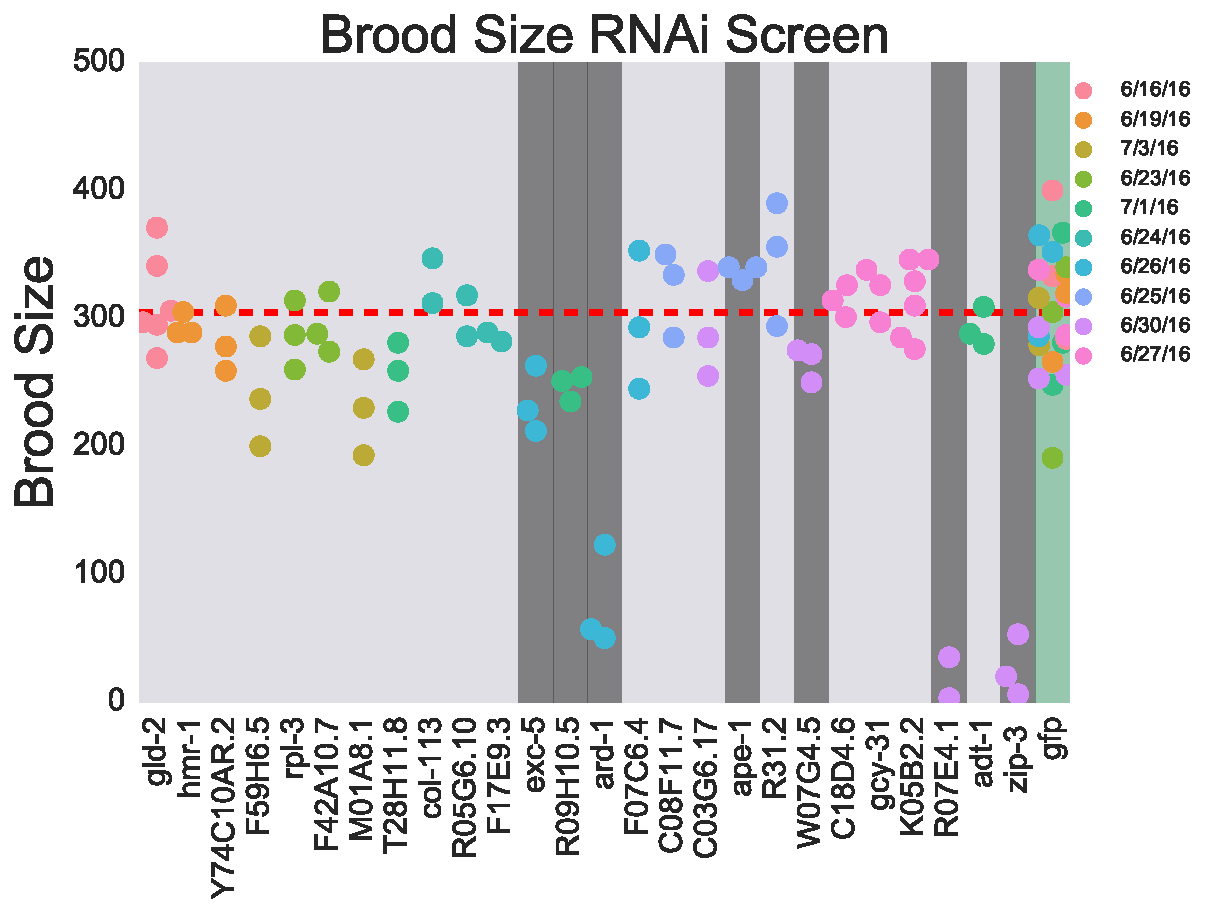
\includegraphics[width=\linewidth]{../output/figs/final_figs/rnai_brood_assay_results.pdf}
% \caption{Brood size screen results. \emph{gfp} control RNAi is shaded in green. Results that are statistically significantly different from \emph{gfp} are shaded in dark grey. Dotted red line shows the mean of the pooled \emph{gfp} controls. Points are colored by the date the assay was started on.
% }%
% \label{fig:broodassay}
% \end{figure}
%
% To test whether the genes we identified might lead to phenotypes when they are perturbed, we performed a series of screens that would identify altered phenotypes associated with sperm loss: fertility, altered lawn-leaving or ovulation rate.
% % Brood Size Screen
% We performed a brood size screen, selecting as targets genes that were upregulated in N2 but downregulated in \fog{}, although we also included a gene that was visually determined to have a brood size phenotype (\emph{zip-3}, which goes down with age). In total, we identified seven genes whose knockdown altered brood size (see Figure~\ref{fig:broodassay}). Most of these genes were associated with decreased brood size. Of the six genes that showed decreased brood size, one had previously been described as having a sterile or lethal phenotype (\emph{ard-1};~\cite{Simmer2003}). Knock-down of \emph{exc-5} had not been described to have a sterile phenotype before.
% The remaining four genes were identified in our screen had not been described previously to have a phenotype. \emph{R09H10.5} and \emph{WO7G4.5} had mild effects on brood size; whereas \emph{zip-3}, and \emph{R07E4.1} had strong effects on fertility. \emph{ard-1}, \emph{R09H10.5} and \emph{WO7G4.5} are all expressed in the intestine.
% Although we cannot rule out that these genes are essential in development, there is a strong functional connection between the intestine and the germline through yolk production~\cite{DePina2011}, and we hypothesize that these genes participate in communication between these tissues in adult worms.
% We also identified \emph{ape-1} as a gene associated with increases in brood size. Given the small effect size, we cannot rule out that this is a false positive, even though we have applied a very conservative methodology to our statistical analysis.
%
% % figure 5 (ovulation assay)
% \begin{figure}
% \renewcommand{\familydefault}{\sfdefault}\normalfont{}
% \centering
% 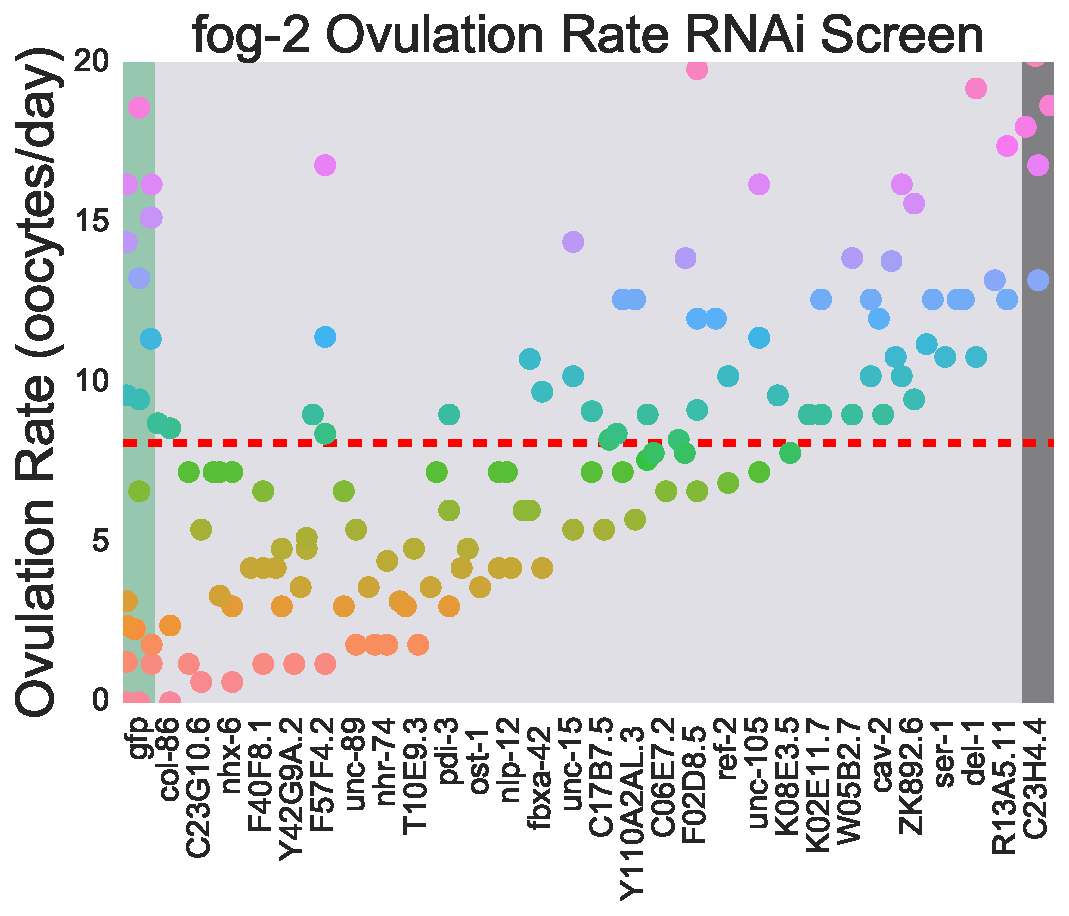
\includegraphics[width=\linewidth]{../output/figs/final_figs/oocyte_rate_assay.pdf}
% \caption{Ovulation Rate Assay. \emph{gfp} control RNAi is shaded in green. Results that are statistically significantly different from \emph{gfp} RNAi are shaded in dark grey. Dotted red line shows the mean of the pooled \emph{gfp} RNAi controls. Points are colored proportionally to their y-coordinate
% }%
% \label{fig:oocytedropping}
% \end{figure}
%
% Some of the genes in our genotype dataset could also be associated with ovulation rate in \fog{}. We selected genes that showed upregulation in \fog{} mutants in our RNA-seq dataset and tested the effect of RNAi treatment against these genes on lawn-leaving behaviour. We observed large variation in the ovulation rate for the control RNAi, and as a result only a single RNAi treatment was associated with alterations in ovulation rate. However, the pooled variance across the screen was very similar to the control variance, suggesting that our failure to identify genes was not a result of poor experimental conditions for a single day/event. Therefore, it is likely the source of variation in our screen was systemic and of equal magnitude across replicates and RNAi strains. Our screen identified a single hit: \emph{C23H4.4,} a predicted carboxyl ester lipase with unknown function.
%
% % figure 4 (lawn-leaving)
% \begin{figure}[htbp]
% \renewcommand{\familydefault}{\sfdefault}\normalfont{}
% \centering
% 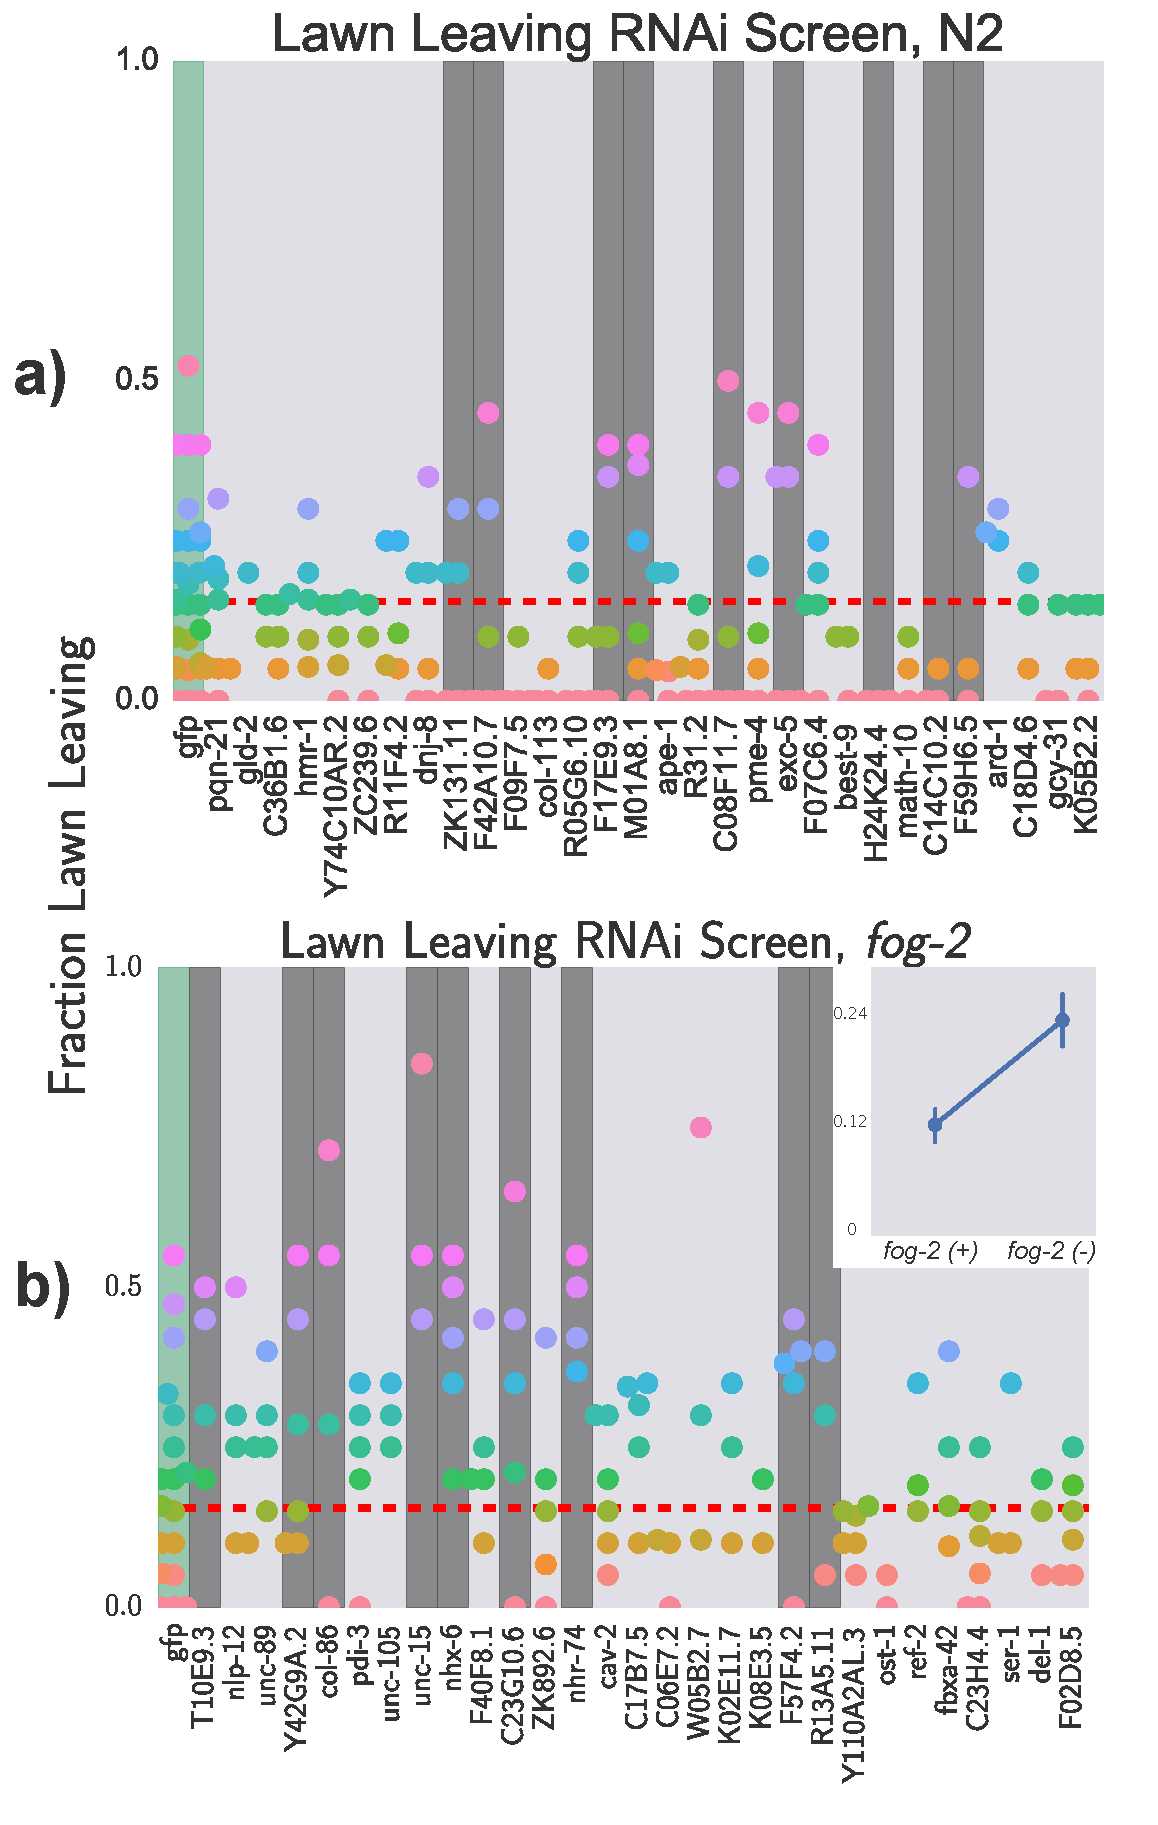
\includegraphics[width=\linewidth]{../output/figs/final_figs/lawn_leaving_rnai_assay.pdf}
% \caption{Lawn-leaving Screen Results. \emph{gfp} control RNAi is shaded in green. Results that are statistically significantly different from \emph{gfp} are shaded in dark grey. Dotted red line shows the mean of the pooled \emph{gfp} controls. Points are colored proportionally to their y-coordinate. \textbf{a} N2 lawn-leaving assay. \textbf{b} \fog{} lawn-leaving assay. Inset shows the screen-wide average lawn-leaving rate of N2 and \fog{}, which shows that the screen-wide lawn-leaving rate of \fog{} worms is twice the rate of lawn-leaving of N2 worms, in agreement with previous literature~\cite{Lipton2004}.
% }%
% \label{fig:lawnleaving}
% \end{figure}
%
% We also performed lawn-leaving assays because previous research has reported differences in hermaphrodite wild-type worms and virgin \fog{} leaving rates, and these differences are believed to be associated with differences in the status of the reproductive system~\cite{Lipton2004}. We tested genes that increased in \fog{} animals in a \fog{} background, expecting that decreasing these genes should lead to a reversal of the lawn-leaving assay. Likewise, we tested genes that were decreased in \fog{} animals in an N2 background, expecting that knockdown of these genes would cause lawn-leaving.
% We identified 9 genes that had an altered lawn-leaving profile in an N2 background, and 9 genes that altered lawn-leaving profile in a \fog{} background. Oddly, both screens identified  genes that mainly stimulate lawn-leaving. Initially, we had expected that RNAi knockdown would allow us to identify genes that inhibit lawn-leaving behavior in an N2 background; whereas RNAi knockdown in a \fog{} background would identify genes that promote lawn-leaving. However, our screen only identified genes that suppress lawn-leaving in an N2 background. All other hits stimulated lawn-leaving.
%
% We also looked for correlations between lawn-leaving phenotypes and ovulation rate in RNAi treated \fog{} worms. This was possible because we used the same worms for both assays. However, we did not find any correlation between the lawn-leaving rate of a worm and ovulation rate (data not shown).
%
% % lawn leaving
% % n2
% % ZK131.11 - pathogen defense
% % F42A10.7 - stress
% % F17E9.3 - nan
% % M01A8.1 - fat content
% % C08F11.7 - nan
% % exc-5 - lethal, dev variant, locomotion variant
% % H24K24.4 - tRNA methyltransferase
% % C14C10.2 - locomotion
% % F59H6.5 - dna helicase, dauer
%
% % fog2
% % T10E9.3 - nan
% % Y42G9A.2 - nan
% % col-86 -cuticle
% % unc-15 - egl
% % nhx-6 - ion channel
% % C23G10.6 - enzyme
% % nhr-74 - tf
% % F57F4.2 - nan
% % R13A5.11 - involved in reproduction

\section*{Discussion}
\label{sec:discussion}

\subsection*{Defining an Early Aging Phenotype}
\label{sub:Defining an Early Aging Phenotype}

Our experimental design enables us to decouple the effects of egg-laying from
aging. As a result, we identified a set of almost 4,000 genes that are altered
similarly between wild-type and \fog{} mutants. Due to the read depth of our
transcriptomic data (20 million reads) and the number of samples measured (3
biological replicates for 4 different life stages/genotypes), this dataset
constitutes a high-quality description of the transcriptomic changes that occur
in any aging population of \cel{} yet published.
Although our data only capture $\sim50\%$ of the expression changes reported
in earlier aging transcriptome literature, this disagreement can be explained
by a difference in methodology; earlier publications typically addressed the
aging of fertile wild-type hermaphrodites only indirectly, or queried aging
animals at a much later stage of their life cycle.


\subsection*{Measurement of a female state is enabled by linear models}
\label{sub:female_state}

We set out to study the self-fertilizing (hermaphroditic) to self-sterile
(female) transition by comparing wild-type animals with \fog{} mutants as they
aged. Our statistical approach enabled us to separate between two biological
processes that are correlated within samples. Because of this intra-sample
correlation, identifying this state via pairwise comparisons would not have been
straightforward. Although it is a favoured method amongst biologists, such
pairwise comparisons suffer from a number of drawbacks.
First, pairwise comparisons are unable to draw on the full statistical power
available to an experiment because they discard almost all information except
the samples being compared. Second, pairwise comparisons require a researcher
to define \emph{a priori} which comparisons are informative. For experiments
with many variables, the number of pairwise combinations is explosively large.
Indeed, even for this two-factor experiment, there are 6 possible combinations
of pairwise comparisons. On the other hand, by specifying a linear regression
model, each gene can be summarized with three variables, each of which can be
analyzed and understood without the need to resort to further pairwise
combinations.

\subsection*{mRNA Levels of Developmental Factors Change Between 1st
             to 6th Day of Adulthood in \cel{}}
\label{sub:development_in_aging}

Our transcriptomes reveal a host of transcription factors that changed between
the 1st and 6th day of adulthood in \cel{}. Many of these transcription factors
have been associated with development via cellular differentiation and
specification. For example, we identified the transcription factor
\emph{lin-32}, which has been associated with neuron
development~\cite{Chalfie1989,Zhao1995,Portman2000}; the Six5 ortholog
\emph{unc-39} has been associated with axonal pathfinding and neuron
migration\cite{Manser1990,Yanowitz2004}; \emph{cnd-1}, a homolog  of the
vertebrate NeuroD transcription factors, is expressed in the early embryo and is
also involved in axon guidance~\cite{Schmitz2007}.
Why these transcription factors increase their expression is a mystery,
but we speculate that this hints at important neuronal changes that are
taking place.
% Such changes might not be unexpected, given changes in behaviour and
% pheromone production that are known to occur as hermaphrodites
% become older~\cite{Morsci2011,Leighton2014}.

Our explorations have shown that the loss of \fog{} partially phenocopies the
transcriptional events that naturally occur as \cel{} ages from the 1st day of
adulthood to the 6th day of adulthood. We interpret this phenocopying as
evidence for a female state in \cel{}.
Given the enrichment of neuronal transcription factors that are associated with
sperm loss in our dataset, we believe this dataset should contain some of the
transcriptomic modules that are involved in these pheromone production and
behavioral pathways, although we have been unable to find these genes.
Currently, we cannot judge how many of the changes induced by loss of
hermaphroditic sperm are developmental (i.e., irreversible), and how many can be
rescued by mating to a male.
While an entertaining thought experiment, establishing whether these
transcriptomic changes can be rescued by males is a daunting experimental task,
given that the timescales for physiologic changes could reasonably be the same
as the timescale of onset of embryonic transcription. All in all, our research
supports the idea that wide-ranging transcriptomic effects of aging in various
tissues can be observed well before onset of mortality, and that \cel{}
continues to develop as it enters a new state of its life cycle.

\subsection*{The \cel{} life cycle, life stages and life states}

% c elegans life cycle
\begin{figure}
\renewcommand{\familydefault}{\sfdefault}\normalfont{}
\centering
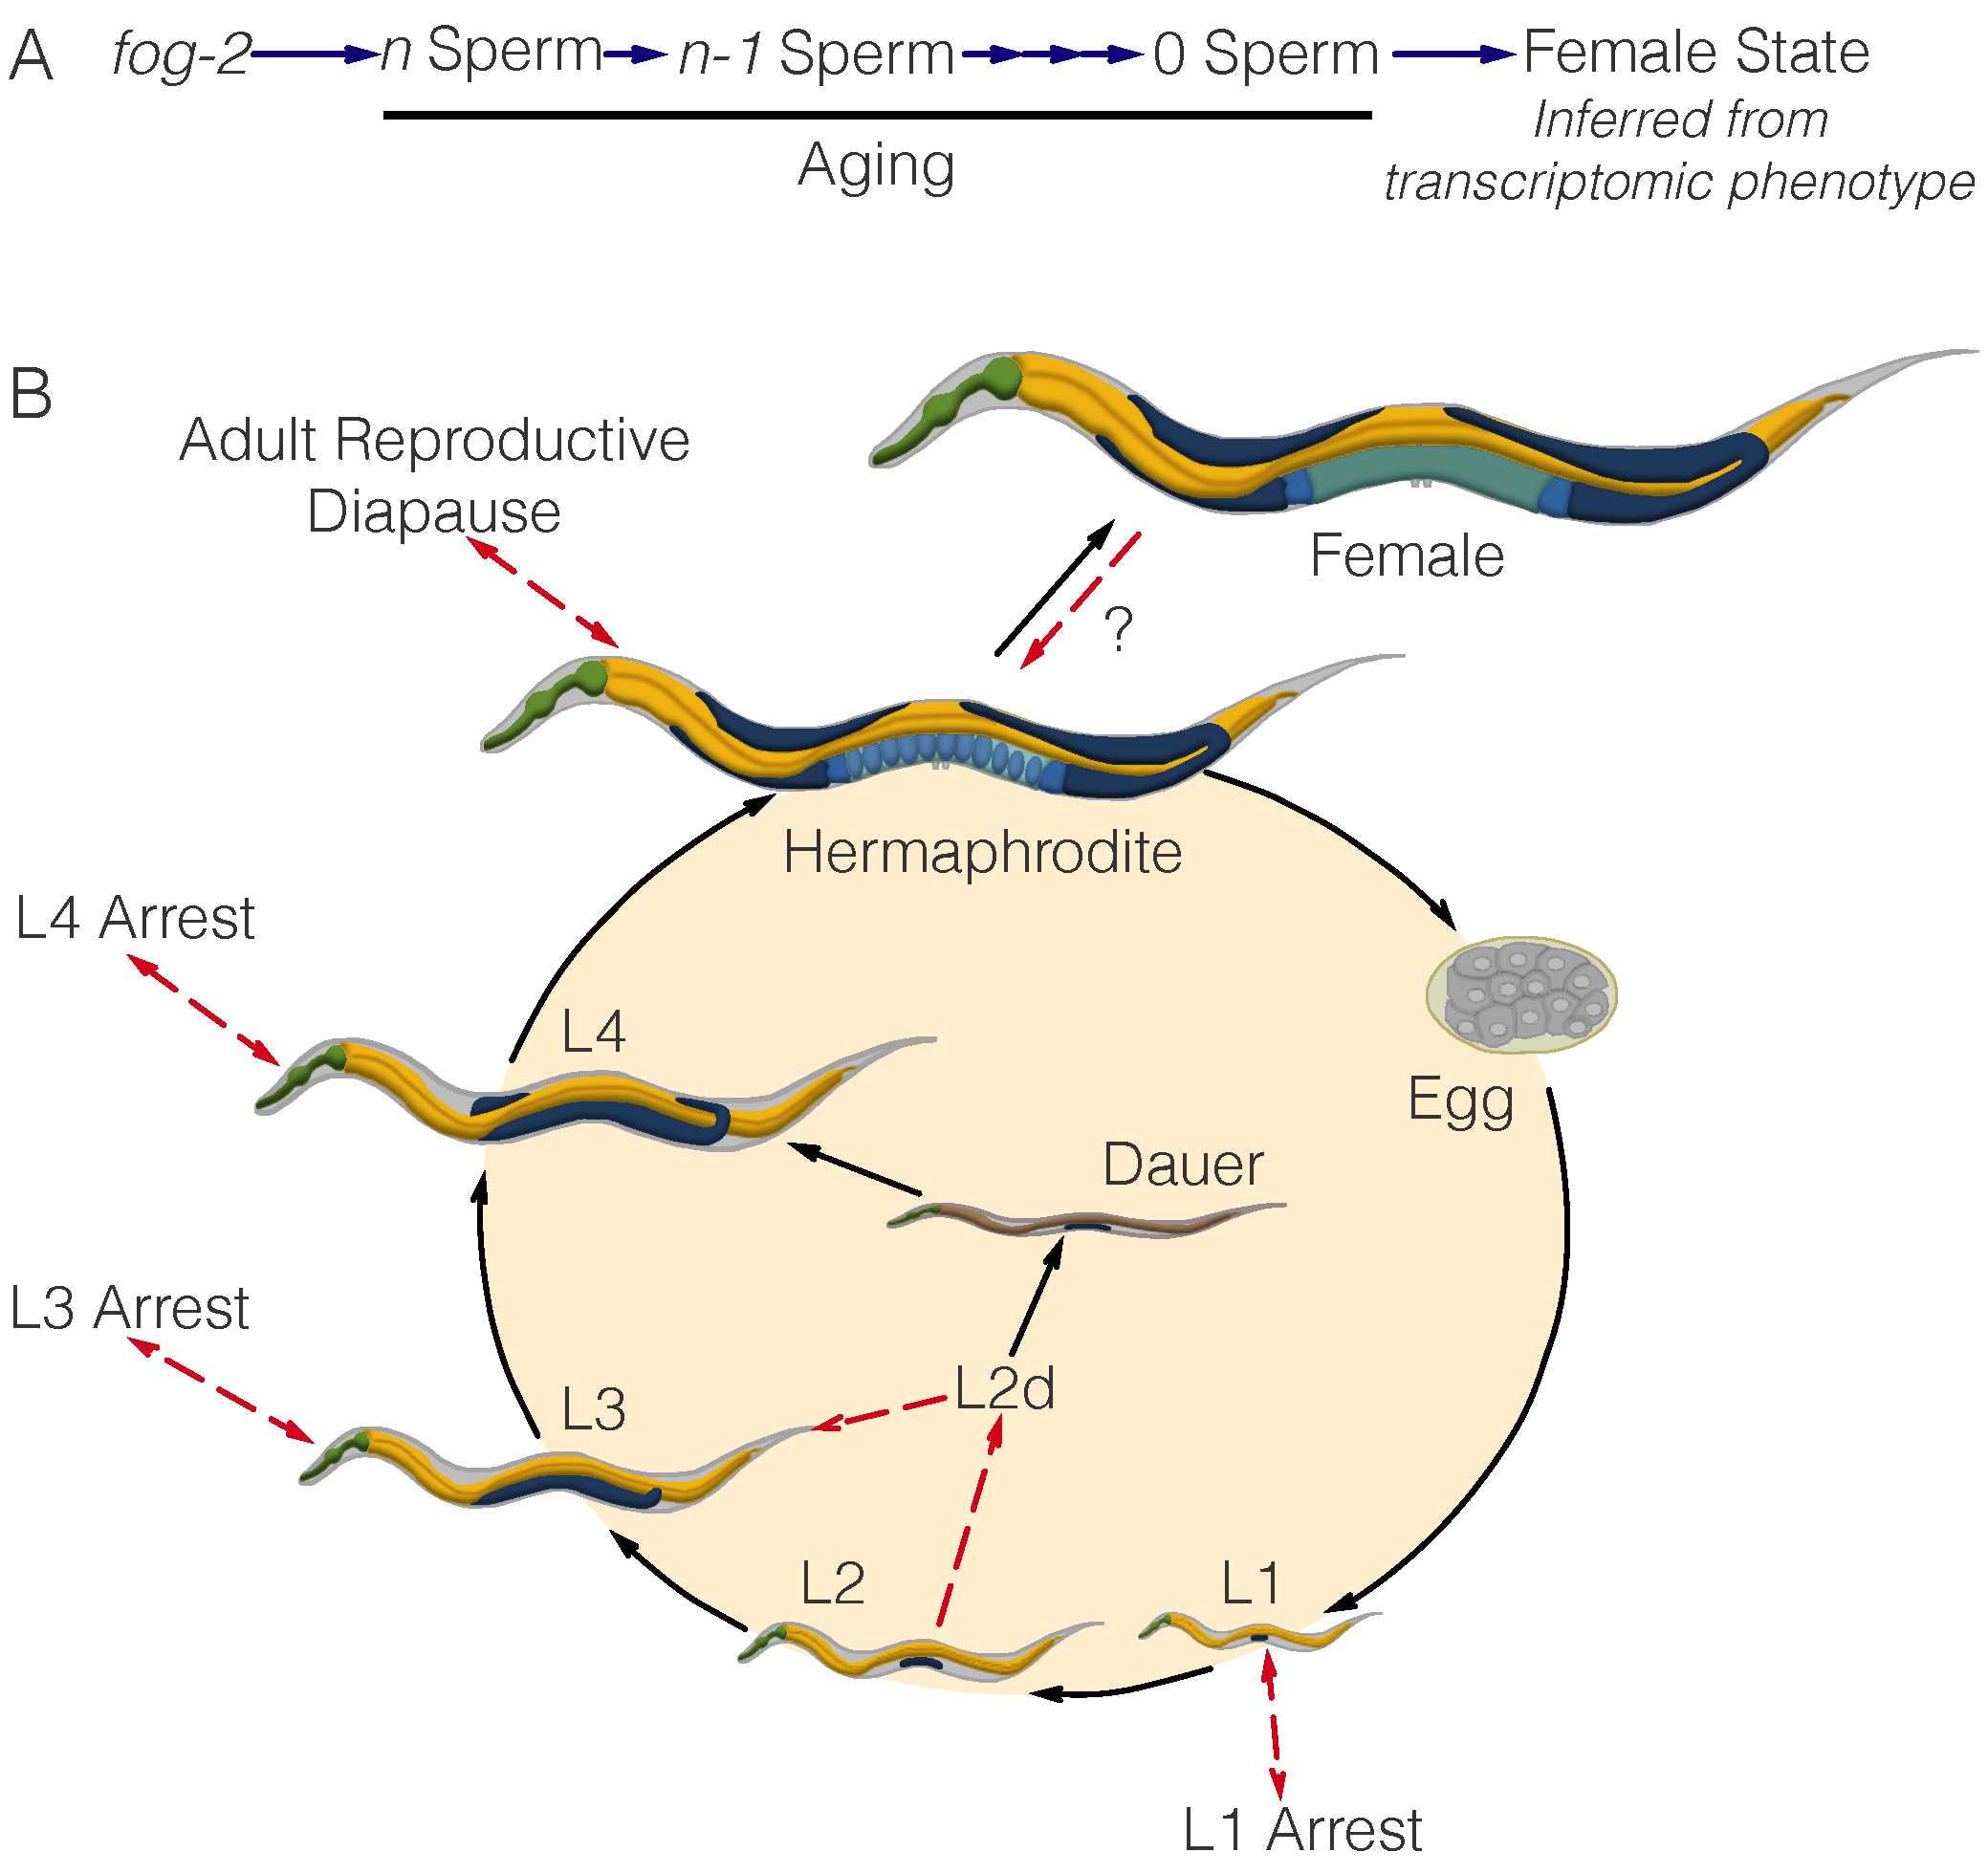
\includegraphics[width=\linewidth]{../output/figs/final_figs/c_elegans_life_cycle.pdf}
\caption{
The complete \cel{} life cycle. Recognized stages of \cel{} are marked by black
arrows. States are marked by red arrows to emphasize that at the end of a state,
the worm returns to the developmental timepoint it was at before entering the
state. The L2d state is an exception. It is the only stage that does not return
to the same developmental timepoint; rather, the L2d state is a permissive state
that allows entry into either dauer or the L3 stage. We have presented evidence
of a female state in \cel{}. At this point, it is unclear whether the difference
between hermaphrodites and females is reversible by males. Therefore, it remains
unclear whether it is a stage or a true state.
}%
\label{fig:lifecycle}
\end{figure}

\cel{} has a complicated life cycle, with two alternative developmental pathways
that have multiple stages (larval development and dauer development), followed
by reproductive adulthood. In addition to its developmental stages, researchers
have recognized that \cel{} has numerous life states that it can enter into when
given instructive environmental cues. One such state is the L1 arrest state,
where development ceases entirely upon starvation~\cite{Johnson1984}. More
recently, researchers have described additional diapause states that the worm
can access at the L3, L4 and young adult stages under conditions of low
food~\cite{Angelo2009,Seidel2011,Schindler2014}. Not all states of \cel{} are
arrested, however (see Fig.~\ref{fig:lifecycle}). For example, the L2d state is
induced by crowded and nutrient poor conditions~\cite{Golden1984}. While within
this state, the worm is capable of entry into either dauer or the L3 larval
stage, depending on environmental conditions. Thus, the L2d state is a
permissive state, and marks the point at which the nematode development is
committed to a single developmental pathway.

Identification of the \cel{} life states has often been performed by
morphological studies (as in the course of L4 arrest or L2d) or via
timecourses (L1 arrest). However, not all states may be visually identifiable,
or even if they are, the morphological changes may be very subtle, making
positive identification difficult. However, the detailed information afforded
by a transcriptome should in theory provide sufficient information to
definitively identify a state, since transcriptomic information underlies
morphology. Moreover, transcriptomics can provide an informative description
into the physiology of complex metazoan life state's via measurements of global
gene expression. By identifying differentially expressed genes and using
ontology enrichment analyses to identify gene functions, sites of expression
or phenotypes that are enriched in a given gene set, researchers can obtain a
clearer picture of the changes that occur in the worm in a less biased manner
than by identifying gross morphological changes.
% To the best of our knowledge, the female state is the first, but and hopefully
% not the last, state in the \cel{} literature to be identified primarily through
% transcriptomic methods.
RNA-seq is emerging as a powerful technology that has been used successfully in
the past as a qualitative tool for target acquisition. More recent work has
successfully used RNA-seq to establish genetic interactions between
genes~\cite{}. In this work, we have shown that RNA-seq data can be analyzed via
linear regression models with interactions to successfully identify internal
states in a multi-cellular organism.

\section*{Acknowledgments}

We thank the \emph{Caenorhabditis} Genetics Center for providing worm strains.
This work would not be possible without the central repository of \cel{}
information generated by WormBase, without which mining the genetic data would
not have been possible. DHWL was supported by a National Institutes of Health
US Public Health Service Training Grant (T32GM07616). This research was
supported by the Howard Hughes Medical Institute, for which PWS is an
investigator.

\subsubsection*{Author Contributions:}
DA, DHWL and PWS designed all experiments. DHWL and THK collected RNA for
library preparation. IA generated libraries and performed sequencing.
DA performed all bioinformatics and statistical analyses.
DA, TT and DHWL performed all screens. DA, DHWL and PWS wrote the paper.

\nolinenumbers{}

%This is where your bibliography is generated.
% Make sure that your .bib file is actually called library.bib
\bibliography{citations}

%This defines the bibliographies style.
% Search online for a list of available styles.
\bibliographystyle{pnas2011}

\end{document}
